\subsection{The assembly-consensus links}

The assembly-consensus link set is a multi-set of links (as in \zcref[S]{definition:link_set}).

A link in this multi-link set is either of two types:
\begin{description}[style=nextline]
  \item[Contig link] A link connecting two fragments from the same contig, thus that can connect:
    \begin{itemize}
      \item two fragments from two contigs of different assemblers
      \item two fragments from two contigs of the same assembler
    \end{itemize}
  \item[Assembly link] A link connecting two fragments from two contigs of the same assembler which were linked in the original assembly graph
\end{description}

\zcref[S]{fig:asmcons_multi-links} illustrates some multi-links cases.

\begin{figure}[htb]
  \centering
  \begin{subfigure}[b]{0.45\linewidth}
    \centering
    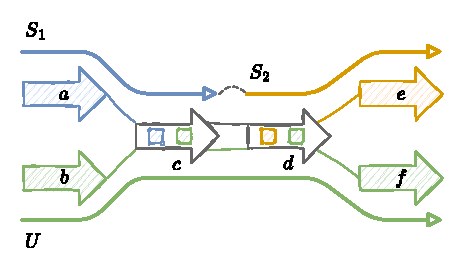
\includegraphics[width=\linewidth]{assembly_consensus_graph/img/panassembly_graph-multi-edges_asm-pan.pdf}
    \caption{Assembly-Contig}\label{subfig:asmcons_asm-pan}
  \end{subfigure}
  \hfill
  \begin{subfigure}[b]{0.45\linewidth}
    \centering
    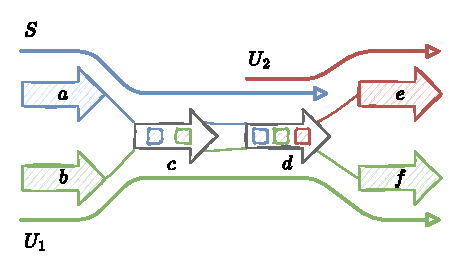
\includegraphics[width=\linewidth]{assembly_consensus_graph/img/panassembly_graph-multi-edges_pan-pan.pdf}
    \caption{Contig-Contig}\label{subfig:asmcons_pan-pan}
  \end{subfigure}
  \figurecaption{Multi-link examples in the assembly-consensus graph.}{%
    Arrows represent (oriented) sequences.
    Heavy ones represent fragments and thin ones represent the contigs.
    %
    \Subref{subfig:asmcons_asm-pan}
    %
    Contig \(U\) comes from Unicycler while contigs \(S_1\) and \(S_2\) come from SKESA.\@
    Fragment set of \(U\) is \( \Fragments(U) = \{b, c, d, f\} \), and these of \(S_1\) and \(S_2\) are respectively \( \Fragments(S_1) = \{a, c\} \) and \( \Fragments(S_2) = \{d, e\} \).
    For example, green link \((c, d) \in \Links{}\) is a contig link while grey link \((c, d) \in \Links{}\) is an assembly link.
    %
    \Subref{subfig:asmcons_pan-pan}
    %
    Contig \(S\) comes from SKESA, defined by \( \Fragments(S) = \{a, c, d\} \), while contigs \(U_1\) and \(U_2\) come from Unicycler, respectively defined by \( \Fragments(U_1) = \{b, c, d\} \) and \( \Fragments(U_2) = \{d, e\} \).
    Both blue and green multi-links \((c, d)\) are contig links, and they respectively connect fragments of contigs \(S\) and \(U_1\).
    However, they enable to connect a subpart of \(U_1\) to contig \(U_2\).
  }\label{fig:asmcons_multi-links}
\end{figure}